\documentclass[usenames,dvipsnames, 18pt, compress, aspectratio=169]{beamer}

% can be compiled by xelatex -shell-escape presentation.tex
% lualatex -shell-escape presentation.tex

\usetheme[]{metropolis}

\usepackage[utf8]{inputenc}
\usepackage[russian, english]{babel}
\usepackage{booktabs}
\usepackage[scale=2]{ccicons}
\usepackage{listings}
\usepackage{marvosym}
\usepackage{color}
\usepackage{xcolor}
\usepackage[document]{ragged2e}
\usepackage[export]{adjustbox}
\usepackage{fontawesome5}
\usepackage{enumitem}
\usepackage{minted}
\usemintedstyle{tango}
\usepackage[normalem]{ulem}
\usepackage{tikz}
\usetikzlibrary{patterns}
\usetikzlibrary{mindmap}
\usetikzlibrary{shapes.misc, fit}
\usetikzlibrary{spy, decorations, decorations.pathmorphing, decorations.pathreplacing, backgrounds, decorations.text}
\usepackage{graphicx}
\usepackage{eso-pic}
\usepackage{verbatim}
\usepackage{smartdiagram}
\usesmartdiagramlibrary{additions}
\usetikzlibrary{trees}
\usepackage{datetime}
\usepackage{hyperref}
\usepackage{forloop}
\usepackage{copyrightbox}
\usepackage{csquotes}
\usepackage{hyperref}
\usepackage{pgfplots}
\usetikzlibrary{tikzmark}
\usetikzlibrary{arrows.meta}

\usepackage{tcolorbox}
\usepackage{tabularx}
\usepackage{array}
\usepackage{colortbl}
\tcbuselibrary{skins}

\usetikzlibrary{shapes,arrows,positioning}
\graphicspath{{images/}}
%\newfontfamily{\FA}{FontAwesome}

\def\social{{\faMastodon}}
\def\github{{\faGithub}}
\def\email{{\faEnvelope}}

\renewcommand{\ttdefault}{pcr}
\setmonofont{FiraCode-VF}
%\newfontfamily{\ttfamily}{FiraCode-VF}

\usefonttheme{professionalfonts} % using non standard fonts for beamer
\usefonttheme{serif} % default family is serif
\usepackage{fontspec}
\setmainfont{Liberation Sans}
\newfontfamily\ExtraLight{Liberation Sans}
\newfontfamily\Light{Liberation Sans}
\newfontfamily\Book{Liberation Sans}
\newfontfamily\Medium{Liberation Sans}

\makeatletter
\newcommand\HUGE{\@setfontsize\Huge{32}{41}}
\makeatother

\newcommand\AtPagemyUpperLeft[1]{\AtPageLowerLeft{%
\put(\LenToUnit{0.85\paperwidth},\LenToUnit{0.05\paperheight}){#1}}}

\newcommand\AtPagemyUpperTop[1]{\AtPageLowerLeft{%
\put(\LenToUnit{0.42\paperwidth},\LenToUnit{0.90\paperheight}){#1}}}

\renewcommand{\ULthickness}{2.0pt}

\definecolor{links}{HTML}{0099FF}
\hypersetup{colorlinks, linkcolor=, urlcolor=links}
\definecolor{greenGood}{HTML}{99FF99}
\definecolor{redBad}{HTML}{FF9980}
\definecolor{title}{HTML}{ee0000}

\setbeamerfont{section title}{family=\Book, size=\Huge, shape=\normalfont}
\setbeamerfont{frametitle}{family=\Book, size=\large, shape=\normalfont}
\setbeamerfont{title}{family=\Book, size=\Large, shape=\normalfont}
\setbeamerfont{subtitle}{size=\small}
\setbeamerfont{author}{family=\ExtraLight, size=\footnotesize}

\definecolor{cec1d24}{RGB}{236,29,36}
\definecolor{cffffff}{RGB}{255,255,255}
\tikzset{>=latex}

\setbeamertemplate{navigation symbols}{}
\beamertemplatenavigationsymbolsempty
\pagenumbering{gobble}

\SetBlockThreshold{0}

\tcbset{
    on line,
    boxsep=4pt,
    left=0pt,
    right=0pt,
    top=0pt,
    bottom=0pt,
    colframe=white
}

\setbeamertemplate{title page}
{

  \vspace*{2.1cm}
  \hspace{5.5cm}
  \begin{minipage}[b][\paperheight]{0.7\textwidth}
  \begin{center}

    \ifx\inserttitle\@empty\else
    {{% \inserttitle is nonempty
      \raggedright%
      %\linespread{1.0}%
      \usebeamerfont{title}%
      \usebeamercolor[fg]{title}%
      %\vspace*{1.3em}
      \if@noSmallCapitals%
        \inserttitle%
      \else%
        \scshape{\color{title} \textbf{\begin{flushleft}\inserttitle\end{flushleft}}}%
      \fi%
      \vspace*{0.3em}
    }}
    \fi

    \vspace*{0.5em}%

    \ifx\insertsubtitle\@empty\else
    {{% \insertsubtitle is nonempty
      \usebeamerfont{subtitle}%
      \usebeamercolor[fg]{subtitle}%
      {\color{black} \insertsubtitle}%
      \vspace*{3.0em}%
    }}
    \fi

    \vspace*{1.0em}%

    \usebeamerfont{author}%
    \usebeamercolor[fg]{author}%
    {\begin{flushleft}\color{black} \insertauthor\end{flushleft}}%

    %\vspace*{1.5em}
    \fontsize{8pt}{10}\selectfont
    {\begin{flushleft}\color{black} 27-06-2023\end{flushleft}}%

    \vfill
    \vspace*{2em}
  \end{center}
  \end{minipage}
}

\setbeamertemplate{section page}
{
  \vspace{2em}
  \centering
  \begin{minipage}{22em}
    \usebeamercolor[fg]{section title}
    \usebeamerfont{section title}
    {\color{black} \insertsectionhead\\[-1ex]}
  \end{minipage}
  \par
}

\setbeamertemplate{footline}
{
\begin{beamercolorbox}[wd=\textwidth,ht=3ex,dp=3ex,leftskip=0.3cm,rightskip=0.3cm]{structure}
  \usebeamerfont{page number in head/foot}
  \insertframenumber
\end{beamercolorbox}
}

\pgfmathdeclarefunction{gauss}{2}{%
  \pgfmathparse{1/(#2*sqrt(2*pi))*exp(-((x-#1)^2)/(2*#2^2))}%
}

\pgfmathdeclarefunction{longtail}{2}{%
  \pgfmathparse{1/(#2*sqrt(2*pi))*exp(-(pow((ln(x)-#1),2))/(2*#2^2))}%
}

\title{Everything Everywhere All at Once: \\ PostgreSQL configuration guide}
\subtitle{}
\date{\today}
\author{DMITRII DOLGOV}
\institute{}

\begin{document}
{
  \usebackgroundtemplate{
\includegraphics[width=\paperwidth]{title.png}}%
  \fontsize{17pt}{18}\selectfont
  \maketitle
}

\AddToShipoutPictureBG{
  \AtPagemyUpperLeft{{
\includegraphics[width=2.0cm,keepaspectratio]{logo.png}}}
}

%\setbeamertemplate{background canvas}{}

\fontsize{17pt}{18}\selectfont

% party tricks references

%{
%\setbeamercolor{background canvas}{bg=black}
%\begin{frame}
    %\frametitle{}
    %\begin{center}
        %\includegraphics[width=1.0\textwidth,center]{nethack.png}
    %\end{center}
%\end{frame}
%\note{Originally about resources, but now not only}
%}

\setbeamertemplate{background canvas}{}

\begin{frame}[fragile]{}
    \centering
    \frametitle{}

    \begin{adjustbox}{width=\textwidth}
    \begin{tikzpicture}
      \node[draw, ultra thick, inner sep=0pt] (img1) {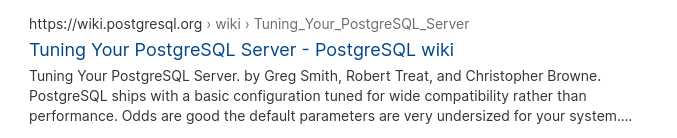
\includegraphics[height=3cm]{tutorial1.png}};
      \pause
      \node[draw, ultra thick, inner sep=0pt] (img2) at (img1.south east) [xshift=-4cm] {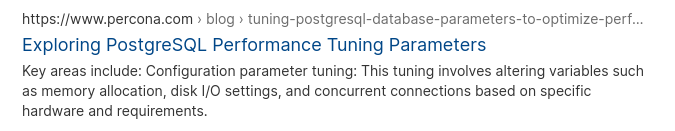
\includegraphics[height=3cm]{tutorial2.png}};
      \pause
      \node[draw, ultra thick, inner sep=0pt] (img3) at (img2.south west) [yshift=-1cm] {
\includegraphics[height=3cm]{tutorial3.png}};
      \pause
      \node[draw, ultra thick, inner sep=0pt] (img4) at (img2.south west) [yshift=1cm, xshift=-0.5cm] {
\includegraphics[height=3cm]{tutorial4.png}};
      \pause
      \node[draw, ultra thick, inner sep=0pt] (img4) at (img1.south) [yshift=-2cm, xshift=3cm] {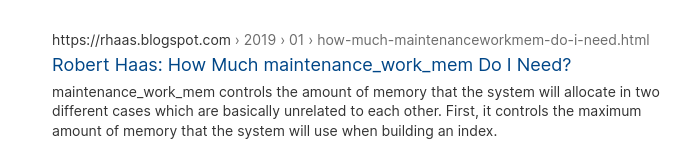
\includegraphics[height=3cm]{tutorial5.png}};
    \end{tikzpicture}
    \end{adjustbox}

\end{frame}

\begin{frame}[fragile]{}
    \frametitle{}
    \begin{center}

		\begin{overprint}[12.5cm]
        \onslide<1>
        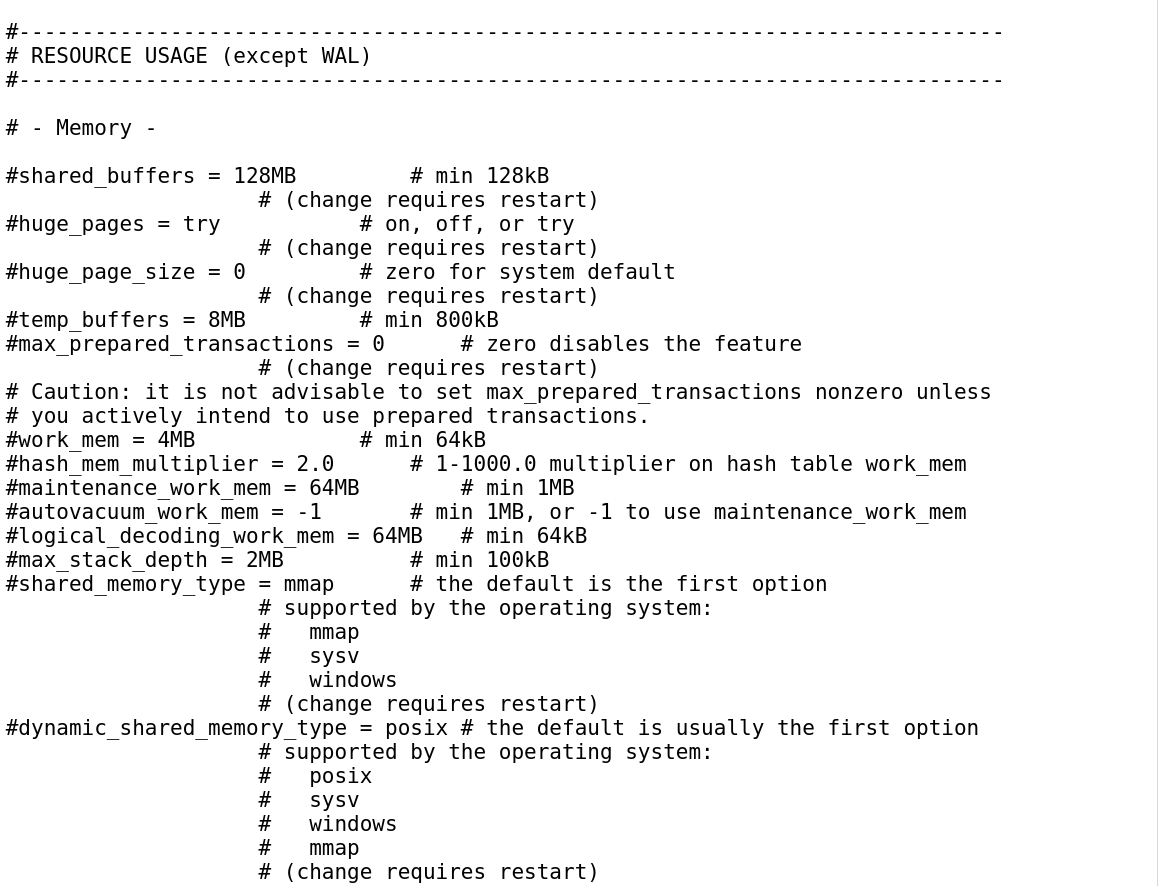
\includegraphics[width=0.9\textwidth,center]{config.png}

        \onslide<2>
        \includegraphics[width=0.9\textwidth,center]{config_elephant.png}

        \onslide<3>
        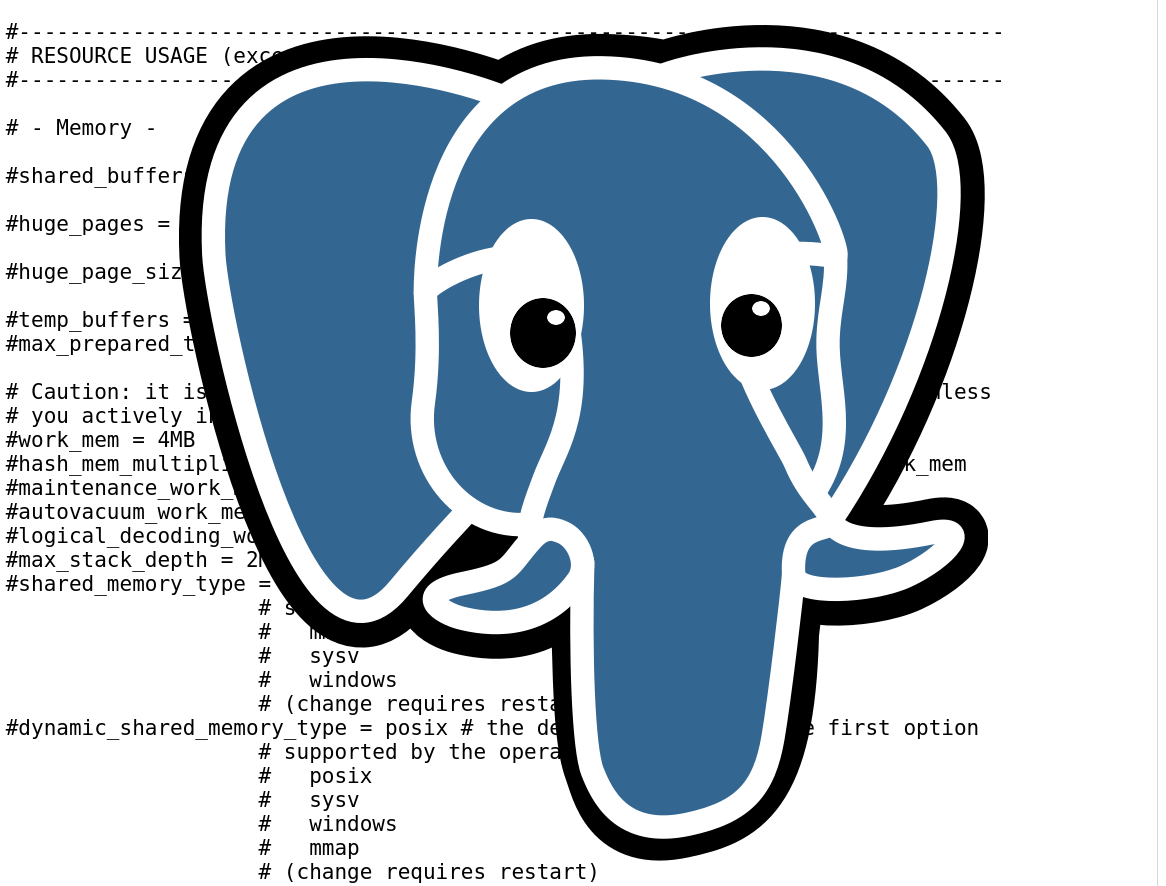
\includegraphics[width=0.9\textwidth,center]{config_elephant_eyes.png}

		\end{overprint}

    \end{center}
\end{frame}
\note{
    Hollistic approach.
}

\section{Types of configuration}

\begin{frame}[fragile]{}
    \frametitle{}
    \begin{center}

        Grand Unified Configuration

    \end{center}
\end{frame}

\begin{frame}[fragile]{}
    \frametitle{}
    \begin{center}

        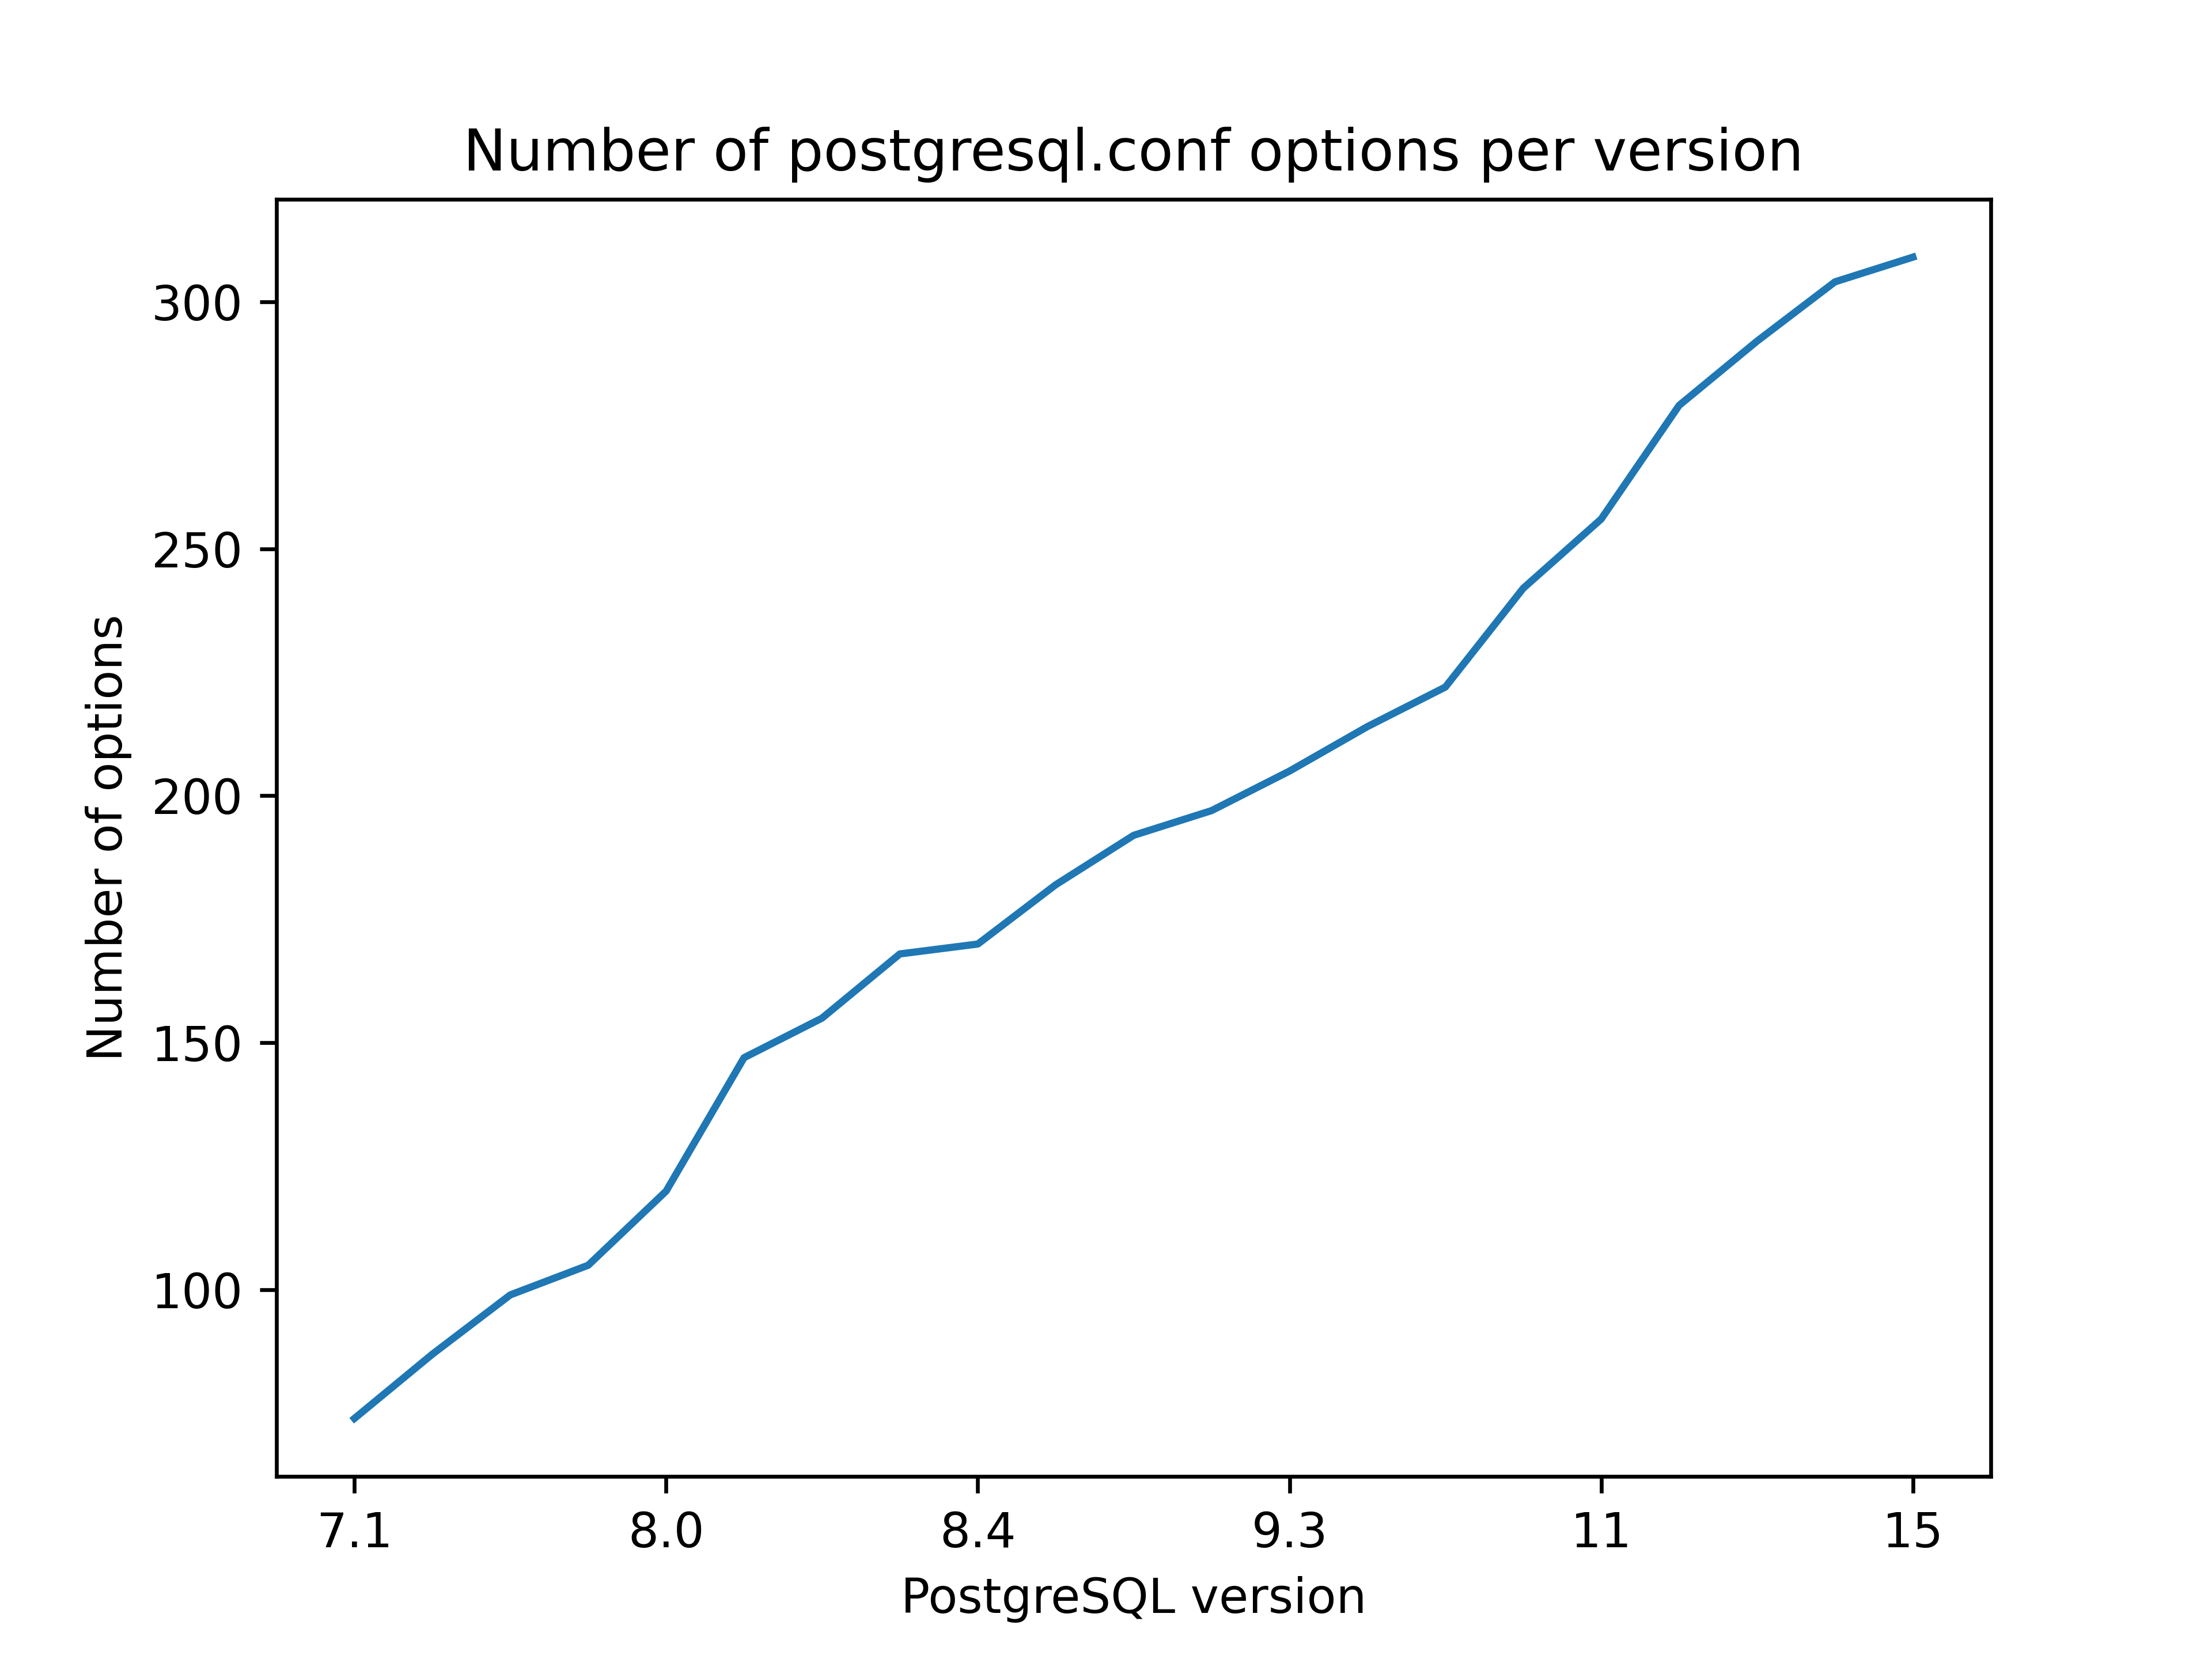
\includegraphics[width=0.8\textwidth,center]{options.png}

    \end{center}
\end{frame}

\begin{frame}[fragile]{}
    \frametitle{}
    \begin{center}

		Postgres95 1.01 Distribution

		\vspace{0.5cm}
        \begin{minted}[fontsize=\large]{c}
           /* ----------------
            *  specify the size of buffer pool
            * ----------------
            */
           NBuffers = atoi(optarg);
        \end{minted}

    \end{center}
\end{frame}
\note {
	Postgres95 1.01 Distribution
}

\begin{frame}[fragile]{}
    \frametitle{}
    \begin{center}

        \blockquote{\it
			[...] one can achieve a substantial portion of the performance gain
			from configurations generated by ML-based tuning algorithms by
			setting two knobs according to the DBMS's documentation. These two
			knobs control the amount of RAM for the buffer pool cache
			and the size of the redo log file on disk.
		}

    \linespread{0.5}
    \vspace{0.5cm}
    \color{black}\fontsize{6pt}{0}\selectfont
		Van Aken, D., Yang, D., Brillard, S., Fiorino, A., Zhang, B., Bilien,
		C. and Pavlo, A., 2021. An inquiry into machine learning-based
		automatic configuration tuning services on real-world database
		management systems. Proceedings of the VLDB Endowment, 14(7),
		pp.1241-1253.
    \linespread{1.5}

    \end{center}
\end{frame}
\note {
    shared_buffers, max_wal_size
}

\begin{frame}[fragile]{}
    \frametitle{}
    \begin{center}

        initdb

		\vspace{0.5cm}
        \begin{minted}[fontsize=\large]{c}
    --wal-segsize=SIZE    size of WAL segments,
                          in megabytes
    --data-checksums      use data page checksums
        \end{minted}

    \end{center}
\end{frame}

\begin{frame}[fragile]{}
    \frametitle{}
    \begin{center}

        "Public" code-based configuration
		\vspace{0.5cm}
        \begin{minted}[fontsize=\large]{shell-session}
    --with-blocksize=8
    --with-wal-blocksize=8
        \end{minted}
        \begin{minted}[fontsize=\large]{c}
    // pg_config_manual.h

    #define PG_CACHE_LINE_SIZE      128
    #define PG_IO_ALIGN_SIZE        4096
    #define NUM_SPINLOCK_SEMAPHORES 128

        \end{minted}

    \end{center}
\end{frame}

\begin{frame}[fragile]{}
    \frametitle{}
    \begin{center}

        "Internal" code-based configuration

		\vspace{0.5cm}
        \begin{minted}[fontsize=\large]{c}
  /*
   * When maintenance_io_concurrency is not saturated,
   * we're prepared to look ahead up to N times
   * that number of block references.
   */
  #define XLOGPREFETCHER_DISTANCE_MULTIPLIER 4
        \end{minted}

    \end{center}
\end{frame}

\begin{frame}[fragile]{}
    \frametitle{}
    \begin{center}

        "Internal" code-based configuration

		\vspace{0.5cm}
        \begin{minted}[fontsize=\large]{c}
  /*
   * Space/time tradeoff parameters: do these need
   * to be user-tunable?
   *
   * To consider truncating the relation, we want
   * there to be at least REL_TRUNCATE_MINIMUM
   * or (relsize / REL_TRUNCATE_FRACTION).
   */
  #define REL_TRUNCATE_MINIMUM	1000
  #define REL_TRUNCATE_FRACTION	16
        \end{minted}

    \end{center}
\end{frame}

\begin{frame}[fragile]{}
    \frametitle{}
    \begin{center}

        "Internal" code-based configuration

		\vspace{0.5cm}
        \begin{minted}[fontsize=\large]{c}
  /*
   * Size of the LRU list.
   *
   * XXX: What's a good value? It should be large
   * enough to hold the maximum number of large
   * tables scanned simultaneously.  But a larger
   * value means more traversing of the LRU list
   * when starting a new scan.
   */
  #define SYNC_SCAN_NELEM 20
        \end{minted}

    \end{center}
\end{frame}

\begin{frame}[fragile]{}
    \frametitle{}
    \begin{center}

        "Internal" code-based configuration

		\vspace{0.5cm}
        \begin{minted}[fontsize=\normalsize]{c}
  /* TODO: Unscientifically determined threshold */
  LLVMPassManagerBuilderUseInlinerWithThreshold(
          llvm_pmb, 512);
        \end{minted}

    \end{center}
\end{frame}

\begin{frame}[fragile]{}
    \frametitle{}
    \begin{center}

        \begin{itemize}
            \item How smart PostgreSQL should be?
            \item How many parameters to expose?
            \item Who is the configuration consumer?
        \end{itemize}

    \end{center}
\end{frame}

\begin{frame}[fragile]{}
    \frametitle{}
    \begin{center}

        "Developer" code-based configuration

		\vspace{0.5cm}
        \begin{minted}[fontsize=\large]{c}
    --enable-profiling
    --enable-debug
    --enable-coverage
    --enable-cassert
        \end{minted}

    \end{center}
\end{frame}

\begin{frame}[fragile]{}
    \frametitle{}
    \begin{center}

        "Developer" code-based configuration

		\vspace{0.5cm}
        \begin{minted}[fontsize=\large]{c}
  /*
   * This assert is too expensive
   * to have on normally ...
   */
  #ifdef CHECK_WRITE_VS_EXTEND
    Assert(blocknum >= mdnblocks(reln, forknum));
  #endif
        \end{minted}

    \end{center}
\end{frame}

\begin{frame}[fragile]{}
    \frametitle{}
    \begin{center}

        "Developer" code-based configuration

		\vspace{0.5cm}
        \begin{minted}[fontsize=\large]{c}
#ifdef CHECK_DEADLOCK_RISK
/*
 * Issue warning if we already hold a lower-level
 * lock on this object and do not hold a lock of
 * the requested level or higher. This indicates
 * a deadlock-prone coding practice.
	        \end{minted}

    \end{center}
\end{frame}

\begin{frame}[fragile]{}
    \frametitle{}
    \begin{center}

        "Developer" code-based configuration

		\vspace{0.5cm}
        \begin{minted}[fontsize=\large]{c}
/* This is just to allow attaching to startup
 * process with a debugger */
#ifdef XLOG_REPLAY_DELAY
  if (ControlFile->state != DB_SHUTDOWNED)
    pg_usleep(60000000L);
#endif
	        \end{minted}

    \end{center}
\end{frame}

\begin{frame}[fragile]{}
    \frametitle{}
    \begin{center}

        "Developer" code-based configuration

		\vspace{0.5cm}
        \begin{minted}[fontsize=\large]{c}
/*
 * This helps detect intermittent faults caused
 * by code that reads a cache entry and then
 * performs an action that could invalidate the
 * entry, but rarely actually does so.  This can
 * spot issues that would otherwise only arise
 * with badly timed concurrent DDL, for example.
 */
#ifdef DISCARD_CACHES_ENABLED

	        \end{minted}

    \end{center}
\end{frame}

\section{System model}

\begin{frame}
    \frametitle{}
    \begin{center}
        \copyrightbox[b]
        {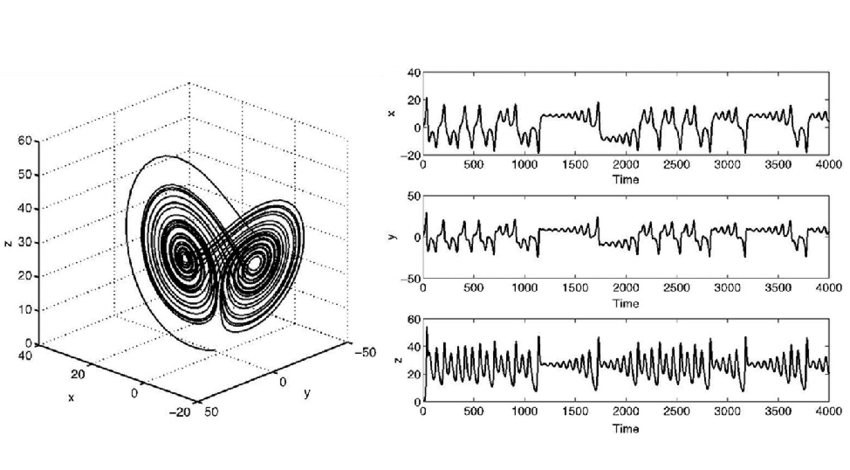
\includegraphics[width=0.8\textwidth,center]{lorenz.png}}
        {
            The phase space plot of the Lorenz attractor, \\
            {\scriptsize
             \color{gray!60}
                 Kuznetsov, N., Bonnette, S. and Riley, M.A., 2013. Nonlinear time series methods\\
                 for analyzing behavioural sequences. In Complex systems in sport (pp. 111-130).}}

    \end{center}
\end{frame}
\note {
    Not only for performance, e.g. for high availability with "recovery time"
    etc.
}

\begin{frame}
    \frametitle{}
    \begin{center}
        Dimensions?

        \begin{itemize}
            \item DB parameters
            \item Hardware resources
            \item Workload parameters
            \item Performance results
        \end{itemize}
    \end{center}
\end{frame}

\section{System dynamics}

\begin{frame}[fragile]{}
    \frametitle{}
    \begin{center}

        \begin{itemize}
            \item Full system model is unknown
            \item Approximate with bunch of simpler models?
            \item Explore the full model experimentally?
        \end{itemize}

    \end{center}
\end{frame}

\begin{frame}[fragile]{}
    \frametitle{}
    \begin{flushleft}

        A simpler model: increase the value of X will lead to better
        performance, but more memory consumption.

    \end{flushleft}
\end{frame}
\note {
    Usually captured in documentation, how-to articles, in a not formalized
    human language.
}

\begin{frame}
    \frametitle{}
    \begin{center}
        \begin{tikzpicture}
        \begin{axis}[
            grid = major,
            xlabel = shared\_buffers,
            ylabel = queries rate,
            zlabel = query latency,
            xtick = \empty,
            ytick = \empty,
            ztick = \empty,
            ticklabel style = {font = \tiny},
            xmajorgrids=false,
            ymajorgrids=false,
            zmajorgrids=false,
            x label style={rotate=-10},
            y label style={rotate=38},
        ]
        \addplot3 [surf, domain=0:180, samples=60]
            { 1 - sin(x) + 0.01 * y };]
        \end{axis}
        \end{tikzpicture}
    \end{center}
\end{frame}

\begin{frame}[fragile]{}
    \frametitle{}
    \begin{center}

        \textbf{A simpler model: more formalized}

        \vspace{0.5cm}
        \begin{itemize}
            \item github.com/le0pard/pgtune
            \item github.com/timescale/timescaledb-tune
            \item github.com/pgconfig/api
            \item github.com/gregs1104/pgtune
        \end{itemize}

    \end{center}
\end{frame}

\begin{frame}[fragile]{}
    \frametitle{}
    \begin{center}
        \copyrightbox[b]
        {
            \includegraphics
            [width=0.4\textwidth,center]
            {engineers.png}
        }
        {
            "The Thrilling Adventures of Lovelace and Babbage", Sydney Padua, 2015
        }

    \end{center}
\end{frame}
\note{
    It's not necessarily bad, more people with knowledge the better. The
    question is how to share the knowledge more efficiently?
}

\begin{frame}[fragile]{}
    \frametitle{}
    \begin{flushleft}

        Simpler model usually do not include
        {{\bf \tcbox[colback=red!30]{higher order}}}
        parameters interaction.

    \end{flushleft}
\end{frame}

\begin{frame}[fragile]{}
    \frametitle{}
    \begin{center}

        \textbf{$2^2$ factorial experiment}

        \vspace{0.5cm}
        \def\arraystretch{1.5}
        \begin{tabular}{|c|c|c|}
          \hline
          \rowcolor{gray!30}
          \cellcolor{gray!30} & A & B \\
          \hline
          \cellcolor{gray!30} (1) & - & - \\
          \hline
          \cellcolor{gray!30} a   & + & - \\
          \hline
          \cellcolor{gray!30} b   & - & + \\
          \hline
          \cellcolor{gray!30} ab  & + & + \\
          \hline
        \end{tabular}

    \linespread{0.5}
    \vspace{0.5cm}
    \color{black}\fontsize{6pt}{0}\selectfont
        Box, G.E., Hunter, J.S. and Hunter, W.G., 2005. Statistics for
        experimenters. \\ In Wiley series in probability and statistics.
        Hoboken, NJ: Wiley.

    \end{center}
\end{frame}
\note{
    Pointer. Add reference to statistic for experimentess.

    ANOVA, factorial design, critical mix.

    Simple example, e.g. shared buffers + work\_mem cause memory pressure?

    More complex example, e.g. shared buffers + io settings (where the
    latter one is kicking in only when the first one is producing bimodal
    latencies).
}

%\begin{frame}[fragile]{}
    %\frametitle{}
    %\begin{center}

        %Simple example, e.g. shared buffers + work\_mem cause memory pressure?

    %\end{center}
%\end{frame}

%\begin{frame}[fragile]{}
    %\frametitle{}
    %\begin{center}

        %More complex example, e.g. shared buffers + io settings (where the
        %latter one is kicking in only when the first one is producing bimodal
        %latencies).

    %\end{center}
%\end{frame}

\begin{frame}[fragile]{}
    \frametitle{}
    \begin{center}

        \textbf{Feedback loop}

        \vspace{1.0cm}
		\begin{overprint}[9cm]
        \onslide<1>
        \begin{tikzpicture}[thick, scale=3, every node/.style={transform shape}]
            \node[draw, ultra thick] (process) {P};
            \coordinate[left=1.5cm of process.center] (input-start);
            \coordinate[right=1.5cm of process.center] (output-start);
            \coordinate[right=0.75cm of process.center] (feedback-start);
            \coordinate[below=0.5cm of process.south west] (corner);
            \coordinate[left=0.5cm of corner] (feedback-middle);
            \coordinate[above=0.2cm of process.south west] (feedback-end);
            \draw[->, thick] (input-start) -- (process) node[fill=white, midway, above] {\tiny Input};
            \draw[->, thick] (process) -- (output-start) node[fill=white, midway, above] {\tiny Output};
            \draw[-, thick] (feedback-start) |- (feedback-middle);
            \draw[->, thick] (feedback-middle) |- (feedback-end);
        \end{tikzpicture}

        \onslide<2>
        \begin{tikzpicture}[thick, scale=3, every node/.style={transform shape}]
            \node[draw, ultra thick] (process) {P};
            \coordinate[left=1.5cm of process.center] (input-start);
            \coordinate[right=1.5cm of process.center] (output-start);
            \coordinate[right=0.75cm of process.center] (feedback-start);
            \coordinate[below=0.5cm of process.south west] (corner);
            \coordinate[left=0.5cm of corner] (feedback-middle);
            \coordinate[above=0.2cm of process.south west] (feedback-end);
            \draw[->, thick] (input-start) -- (process) node[fill=white, midway, above] {\tiny Input};
            \draw[->, thick] (process) -- (output-start) node[fill=white, midway, above] {\tiny Output};
            \draw[-, thick] (feedback-start) |- (feedback-middle) node[draw, fill=white, pos=0.725] {\tiny Ctrl};
            \draw[->, thick] (feedback-middle) |- (feedback-end);
        \end{tikzpicture}

		\end{overprint}

    \end{center}
\end{frame}
\note{
    Scale is important.
    "Self-driving", but not on the whole database level, rather on the smaller
    scale.
    Identify important feedback sources, limiting resources.
    It's not a full fleged ML on top of the db. ML for db tuning, like
    Ottertune, will bring a lot of real-world problems to deal with.
}

\begin{frame}[fragile]{}
    \frametitle{}
    \begin{center}

        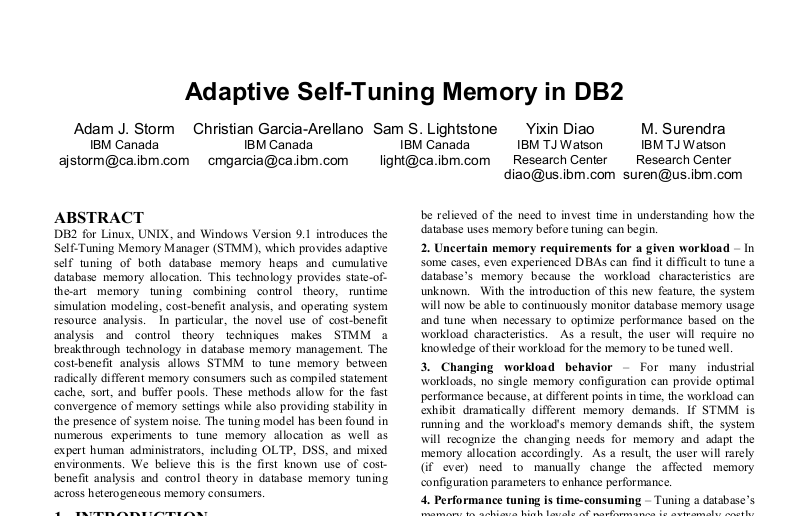
\includegraphics[width=0.8\textwidth,center]{db2.png}

    \end{center}
\end{frame}
\note {
    Example with memory control thread
}

\section{System stability}

\begin{frame}[fragile]{}
    \frametitle{}
    \begin{center}

        Is highest performance enough?

    \end{center}
\end{frame}

\begin{frame}
    \frametitle{}
    \begin{center}
		\begin{overprint}[9cm]

        \onslide<1>
        \begin{tikzpicture}
        \begin{axis}[
            grid = major,
            xlabel = param A,
            ylabel = workload B,
            zlabel = query latency,
            xtick = \empty,
            ytick = \empty,
            ztick = \empty,
            ticklabel style = {font = \tiny},
            xmajorgrids=false,
            ymajorgrids=false,
            zmajorgrids=false,
            opacity=0.8,
            x label style={rotate=-10},
            y label style={rotate=38},
            %x label style={at={(axis description cs:0.5,-0.1)}, anchor=north},
            %view={60}{30},
            %view/az=14,
        ]
        \addplot3 [surf, samples=60]
            { - exp(-sqrt(x^2 + y^2)) };
        \addplot3+[mark size=0.1mm, scatter, domain=0:5*pi, samples=20, samples y=0]
            ({0.3 * sin(deg(x))}, {0.3 * cos(deg(x))}, {-1.0});
        \end{axis}
        \end{tikzpicture}

        \onslide<2>
        \begin{tikzpicture}
        \begin{axis}[
            grid = major,
            xlabel = param A,
            ylabel = workload B,
            zlabel = query latency,
            xtick = \empty,
            ytick = \empty,
            ztick = \empty,
            ticklabel style = {font = \tiny},
            xmajorgrids=false,
            ymajorgrids=false,
            zmajorgrids=false,
            opacity=0.8,
            x label style={rotate=-10},
            y label style={rotate=38},
            %view={60}{30},
            %view/az=14,
        ]
        \addplot3 [surf, samples=60]
            { - exp(-sqrt(x^2 + y^2)) };
        \addplot3+[mark size=0.1mm, scatter, domain=0:5*pi, samples=90, samples y=0]
            ({3.0 * sin(deg(x))}, {3.0 * cos(deg(x))}, {-1.0});
        \addplot3+[mark size=0.1mm, scatter, domain=0:5*pi, samples=60, samples y=0]
            ({2.0 * sin(deg(x))}, {2.0 * cos(deg(x))}, {-1.0});
        \addplot3+[mark size=0.1mm, scatter, domain=0:5*pi, samples=40, samples y=0]
            ({0.8 * sin(deg(x))}, {0.8 * cos(deg(x))}, {-1.0});
        \addplot3+[mark size=0.1mm, scatter, domain=0:5*pi, samples=20, samples y=0]
            ({0.3 * sin(deg(x))}, {0.3 * cos(deg(x))}, {-1.0});
        \end{axis}
        \end{tikzpicture}

		\end{overprint}

    \linespread{0.5}
    \vspace{0.5cm}
    \begin{flushleft}
    \color{black}\fontsize{6pt}{0}\selectfont
        Huynh, A., Chaudhari, H.A., Terzi, E. and Athanassoulis, M., 2021.
        Endure: A Robust Tuning Paradigm for LSM Trees Under Workload
        Uncertainty. arXiv preprint arXiv:2110.13801.
    \linespread{1.5}
    \end{flushleft}

    \end{center}
\end{frame}
\note {
    Academia, rocksdb.

    Put workload B axis more precise.
}

\section{Final thoughts}

\begin{frame}[fragile]{}
    \frametitle{}
    \begin{center}

        \begin{itemize}
            \item Who's using?
            \item           An engineer or an algorithm.
            \item
            \item What's missing?
            \item           Higher-order interaction and feedback.
            \item
            \item What's the goal?
            \item           Best robust performance.
        \end{itemize}

    \end{center}
\end{frame}

\fontsize{18pt}{18}\selectfont
\begin{frame}
  \vspace*{2.5cm}
  \begin{minipage}[b][\paperheight]{\textwidth}
  \begin{center}

      %\raggedright%
      \linespread{1.0}%
      \usebeamerfont{title}%
      \usebeamercolor[fg]{title}%
      \if@noSmallCapitals%
        Questions?
      \else%
        \scshape{\color{black} Questions?}%
      \fi%
      \vspace*{0.3em}

      \usebeamerfont{subtitle}%
      \fontsize{13pt}{14}\selectfont
      \usebeamercolor[fg]{subtitle}%
        \begin{itemize}[label={}]
            \item {\color{black} \social\ @erthalion@fosstodon.org}
            \item {\color{black} \email\ ddolgov at redhat dot com}
        \end{itemize}
      \vspace*{2.5em}%

    \vfill
    \vspace*{2em}
  \end{center}
  \end{minipage}

\end{frame}

\end{document}
